\documentclass{article}
\usepackage[en]{homework}
\usepackage{tikz}

\config{Physics-0}{2026 Spring}{9}

\begin{document}

\begin{problem}
(30pts) Consider an infinitely long cylindrical shell of inner and outer radii $r_1$ and $r_2$, with uniform charge density $\rho$. Use Gauss' law to find the electric field
\begin{enumerate}[label=(\alph*)]
    \item (10pts) Outside the shell where $|\bo{r}| > r_2$
    \item (10pts) At a position $\bo{r}$ where $r_2 > |\bo{r}| > r_1$
    \item (10pts) Inside the shell where $r_1 > |\bo{r}|$
\end{enumerate}
\end{problem}

\begin{solution}
  By the symmetry of the problem, the electric field must be the form of \( \bo{E}=E(r) \hat{\bo{r}} \), where \( r=|\bo{r}| \). Choose a surface of a cylinder of radius \( r \) and length \( L \) as the Gaussian surface. The total charge enclosed by the Gaussian surface is given by
  \[ Q(r)=\begin{cases}
    0,& r<r_1\\
    \rho\pi (r^2-r_1^2)L, & r_1<r<r_2\\
    \rho\pi (r_2^2-r_1^2)L, & r>r_2
  \end{cases} \]

  By the Gauss' law, we have
  \[ 2\pi r L E(r) = \frac{Q(r)}{\varepsilon_0}, \]
  and hence
  \[ \bo{E}(r) = \begin{cases}
    0, & r<r_1 \\
    \frac{\rho (r^2-r_1^2)}{2\varepsilon_0 r}\hat{\bo{r}}, & r_1<r<r_2 \\
    \frac{\rho (r_2^2-r_1^2)}{2\varepsilon_0 r}\hat{\bo{r}}, & r>r_2
  \end{cases} \]
\end{solution}



\begin{problem}
(20pts) In two spatial dimensions, Gauss' law is given in terms of the line integral
\[
\int_{\partial M} \bo{E} \cdot \hat{\bo{n}} \, \d l = 2\pi\tilde{k}Q
\]
where the integral is over a piecewise smooth curve $\partial M$ (the boundary of a two-dimensional surface $M$), $\hat{\bo{n}}$ is the vector normal to the curve, $\tilde{k}$ is the two-dimensional Coulomb's constant, and $Q$ is the total charge enclosed by the curve $\partial M$.

Compute the electric field of an infinite line with uniform linear charge density $\lambda$ using Gauss' law and compare this result with the one obtained in problem (3b) of the previous homework.
\end{problem}

\begin{solution}
  Consider the line lying at \( x \)-axis. By the symmetry of the problem, the electric field must be the form of \( \bo{E}(x,y)=\operatorname{sgn}(y) E(|y|)\hat{\bo{y}} \). Choose a retangle with \( 4 \) vertices at \( (\pm L,\pm H) \). The total charge enclosed by the rectangle is given by \( Q=2\lambda L \). By the Gauss' law, we have
  \[ 4L E(y) = 2\pi\tilde{k}Q = 2\pi\tilde{k}(2\lambda L) \]
  and hence
  \[ E(y) = \pi\tilde{k}. \]

  Therefore, the electric feild is given by
  \[ \bo{E} = \operatorname{sgn}(y) \pi\tilde{k} \hat{\bo{y}} \]
\end{solution}



\begin{problem}
(40pts) Consider a line along the $z$ axis of length $L$ and uniform linear charge density $\lambda$. It's convenient to use polar coordinates on the $xy$-plane such that $(x,y,z) = (r_2 \cos\theta, r_2 \sin\theta, z)$.

\begin{figure}[H]
    \centering
    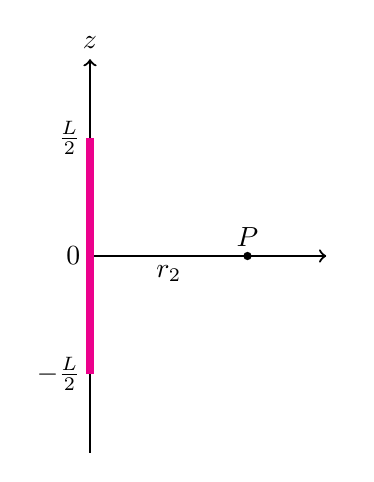
\begin{tikzpicture}
        % Axes
        \draw[->, thick] (0,-2.5) -- (0,2.5) node[above] {$z$};
        \draw[->, thick] (0,0) -- (3,0) node[right] {};
        
        % Line charge
        \draw[line width=3pt, magenta] (0,-1.5) -- (0,1.5);
        
        % Labels
        \node[left] at (0,1.5) {$\frac{L}{2}$};
        \node[left] at (0,-1.5) {$-\frac{L}{2}$};
        \node[left] at (0,0) {$0$};
        
        % Point P
        \fill (2,0) circle (1.5pt) node[above] {$P$};
        \node[below] at (1,0) {$r_2$};
    \end{tikzpicture}
\end{figure}

\begin{enumerate}[label=(\alph*)]
    \item (10pts) Compute the electric potential $\varphi(r_2)$ at the point $P$, located on the $xy$-plane at $z=0$ a distance $r_2$ from the line of charge.
    \item (5pts) Compute the $r_2$ component of the electric field at the point $P$. Is the result compatible with the result of problem (2a) of the previous homework?
    \item (10pts) To obtain the electric potential of an infinitely long line you may want to send $L \to \infty$. However, the answer is divergent! Explain the reason why.
    \item (10pts) You can obtain a finite result by first computing the difference $\varphi(r_2) - \varphi(r'_2)$ where $r'_2 \neq r_2$ is another position in the $xy$-plane, and then take the $L \to \infty$ limit. Write down the result and explain why this works.
    \item (5pts) Use the electric potential obtained above to compute the electric field at $P$. Check that your result matches the electric field we found in class.
\end{enumerate}
\end{problem}

\begin{solution}
  (a) The electric potential at the point \( P \) is given by
  \begin{align*}
    \varphi(r_2)
    &=\int_{-L/2}^{L/2}\frac{1}{4\pi \varepsilon_0} \frac{\lambda \d z}{\sqrt{r_2^2 + z^2}}
    =\int_{-\arctan(L/2r_2)}^{\arctan(L/2r_2)}\frac{\lambda r_2}{4\pi\varepsilon_0}\frac{\d\tan\theta}{r_2\sec\theta}
    =\frac{\lambda}{4\pi\varepsilon_0}\left.\ln\abs{\frac{1+\sin\theta}{\cos\theta}}\right|^{\arctan(L/2r_2)}_{-\arctan(L/2r_2)}\\
    &=\frac{\lambda}{2\pi\varepsilon_0}\ln\left( \frac{L+\sqrt{L^2+4r_2^2}}{2r_2} \right)
  \end{align*} 

  (b) The \( r_2 \) component of the electric field at the point \( P \) is given by
  \begin{align*}
    E_r(r_2) &= -\frac{\partial \varphi}{\partial r_2} 
    =-\frac{\lambda}{2\pi\varepsilon_0}\left( \frac{1}{L+\sqrt{L^2+4r_2^2}}\frac{8r_2}{2\sqrt{L^2+4r_2^2}}-\frac{1}{r_2} \right)\\
    &=\frac{\lambda}{2\pi\varepsilon_0}\frac{\left( L\sqrt{L^2+4r_2^2}+L^2+4r_2^2 \right)-4r^2}{r_2\sqrt{L^2+4r_2^2}\left( L+\sqrt{L^2+4r_2^2} \right)}\\
    &=\frac{\lambda}{2\pi\varepsilon_0}\frac{L}{r_2\sqrt{L^2+4r_2^2}}.
  \end{align*}

  This result agrees with the result of problem (2a) of the previous homework.

  (c) This is because the zero point of the electric potential is defined by the infinity, but the electric potential of an infinite line is divergent at infinity (since the charge is distributed in an infinite large space).

  (d) The difference of the electric potential is given by
  \[ \varphi(r_2) - \varphi(r'_2)=\frac{\lambda}{2\pi\varepsilon_0}\ln\left( \frac{L+\sqrt{L^2+4r_2^2}}{L+\sqrt{L^2+(r_2')^2}}\frac{2r_2'}{2r_2} \right)=-\frac{\lambda}{2\pi\varepsilon_0}\ln\frac{r_2}{r_2'}.\quad (L\to\infty) \]

  (e) The electric field at \( P \) is given by
  \[ E_r(r_2)=-\frac{\partial \varphi}{\partial r_2}=\frac{\lambda}{2\pi\varepsilon_0}\frac{1}{r_2}, \]
  which matches the electric field we found in class.
\end{solution}



\begin{problem}
(10pts) An electron moves with a speed of $6 \times 10^6 \mathrm{ m/s}$ in a direction perpendicular to the Earth's magnetic field, which has a strength of $5 \times 10^{-5} \mathrm{ T}$. What electric field strength must be applied perpendicular to the Earth's magnetic field to make the electron move in a straight line?
\end{problem}

\begin{solution}
  To make the Lorentz and Coulomb forces cancel each other, we have
  \[ eE = evB \]
  and hence
  \[ E = vB = 6 \times 10^6 \mathrm{ m/s} \times 5 \times 10^{-5} \mathrm{ T} = 300 \mathrm{ V/m}. \]
\end{solution}

\end{document}